\chapter{序論}
\label{introduction}

本章では本研究の背景,課題及び手法を提示し,本研究の概要を示す.

\section{インターネットを介した音楽演奏への注目}
世界的なインターネット,SNSの普及がもたらしたグローバルなコミュニケーションの発展により,世界中のアーティストをつなぐグローバルな音楽のコミュニティが形成している.
私自身も作曲者,ベース演奏者,DJとして様々な方面でこれらのコミュニティに活発に参加している.

従来まではこのようなインターネットを介したコミュニティでは音楽演奏を共有する手段として,事前に音楽演奏を録音し,ファイル共有サービスなどを用いて音声データを送り合うしかなかった.
バンド,楽団など複数人の同時に合奏を行う音楽形式ではこのような音声データを集めたのち,一人が演奏音声を合成し一つの楽曲として聞ける形に変換するという手段が主流である.
しかしSkypeやZoomなどのVoIPアプリケーションが普及し,インターネットを介したリアルタイムの音楽演奏が現実的になってきた.
このような音楽演奏を「ネットワーク音楽演奏 (Network Music Performance)\cite{lazzaro}\cite{nmpbook}」と呼ぶ.

その状況の中,2020年の新型コロナウイルス感染症が流行し現実で集まった生演奏が難しくなり,このような演奏形式が益々注目されるようになった.
この時期にYamahaは低遅延でネットワーク音楽演奏を行えるSyncroom\cite{syncroom}\cite{syncroom:press}を発表し,2023年6月に株式会社ズームはネットワーク音楽演奏が行えるデバイスS6 SessionTrak\cite{sessiontrak}を発表するなど,直近でもこのネットワーク音楽演奏に対する注目度は高まっていることがわかる.

\section{遅延の問題}
ネットワーク音楽演奏において遅延は致命的な問題である.
リアルタイムで相手の演奏に同期して自らの演奏を行う必要があるネットワーク音楽演奏において,このプロセスへの遅延は演奏に多大な影響を与える.
この効果は様々な研究で観測され,様々な演奏環境により差があれど遅延時間に差があれど20〜40ms以上で遅延を感じることができ,80〜100ms以上になると演奏が不可能になるとされている\cite{latency:effect}\cite{latency:ipsj}.

\subsection{遅延のモデル}
音楽演奏は一定の「拍子」で行われ,各演奏者は相手の演奏を聴き,拍子を認識し,その拍子に合わせて演奏を行う.
単独で演奏を行う奏者は一つのオシレータのように一定の間隔で刻まれる拍に合わせて音を配置していると捉えることができる.
この場合遅延がある二人同士のネットワーク音楽演奏は\ref{fig:oscillator}のように錬成振動のモデルで捉えられる.

\begin{figure}
  \centering
  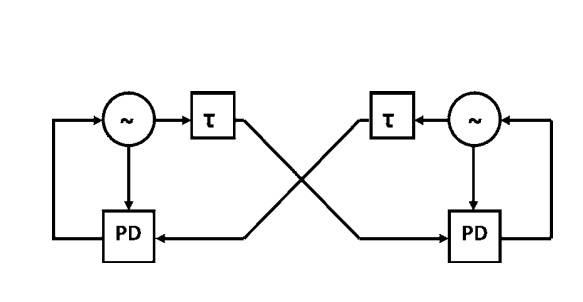
\includegraphics[width=0.8\linewidth]{src/latencymodel.png}
  \caption{連成振動のモデル.\cite{latency:model}より引用}
  \label{fig:oscillator}
\end{figure}

ここでPDはPhase Detector,すなわち演奏者の捉えた拍の感覚,\begin{math}\tau\end{math}は遅延時間である.
\cite{latency:model}\cite{nmp:overview}ではこのモデルを踏まえて遅延下の2人の演奏者同士が合意するテンポを以下のように表した.

\begin{displaymath}
  \Omega_{i+1} = \frac{\omega_i }{1 + k\tau}
\end{displaymath}

\begin{math}\omega \end{math}は両演奏者の平均テンポ,kは振動の状態更新を表す低数であり,\begin{math}\tau \end{math}は遅延を表す.
この通り遅延が大きくなると演奏テンポが楽曲を通して遅くなることがわかり,\cite{latency:ipsj}などの遅延つきのネットワーク音楽演奏の実験でもこの傾向は観察できる.

\section{問題提起,目的}
ネットワーク音楽演奏における遅延の課題について説明してきたが,すでにYamahaのSyncroom\cite{syncroom}に代表される遅延の軽減システムは多数存在する.
しかし遅延には様々な原因\cite{nmp:overview}があり,中には避けられないものもある.
例えば本論文執筆時現在,東京からロサンゼルス間のネットワーク遅延は\cite{wondernetwork}によると約107msあり,前述の指標によるとリアルタイムの演奏が不可能である.
この通信は東京からロサンゼルス間の距離,太平洋を渡る海底ケーブルに制限されていて技術の向上での改善はのぞみづらい.
グローバルなネットワーク音楽演奏を前提とするとこのような遅延は必然で,減らすという手法は限界がある.
Syncroomなどのシステムはいずれも「日本国内」に利用を限定させていて,グローバルな演奏はスコープ外としている.

本研究では大きな遅延を前提として,遅延を減らすのではなく,遅延がある中でも快適に演奏を行うシステムを目指す.
その手法としてリズム予測を用いて実質的な無遅延のネットワーク音楽演奏システムを提案する.


\section{本論文の構成}

本論文における以降の構成は次の通りである.

~\ref{background}章では,背景と関連研究を述べる.
~\ref{proposed}章では,本研究の提案手法を述べる.
~\ref{implementation}章では,~\ref{proposed}章で述べたシステムの実装について述べる.
~\ref{evaluation}章では,本システムの実験評価を行い,考察する.
~\ref{conclusion}章では,本研究のまとめと今後の課題についてまとめる.


%%% Local Variables:
%%% mode: japanese-latex
%%% TeX-master: "../thesis"
%%% End:
